\documentclass[11pt]{article}

\usepackage{amsfonts}
\usepackage{fancyvrb}
\usepackage{url}
\usepackage{graphicx}
\usepackage{caption}
\usepackage{subcaption}
\usepackage{dsfont}

\setlength{\oddsidemargin}{0in}
\setlength{\evensidemargin}{0in}
\setlength{\textwidth}{6.5in}
\setlength{\topmargin}{0in}
\setlength{\headsep}{0.5in}
\setlength{\textheight}{8.5in}
\setcounter{page}{1}
%\pagestyle{empty}
%\hbadness=10000

\begin{document}
\huge
\noindent
{Discrete Optimization Assignment:}
\vspace{0.25cm}

\noindent
{\bf Set Cover}
\normalsize

\section{Preamble}

This is an open source assignment and will not count toward your final grade in the course.  This assignment looks-and-feels like all of the other assignments in the class, but you may ignore the typical collaboration policy guidelines and share your source code with your classmates.

To foster code sharing on this assignment, we provide a github repository including various solutions to this problem (\texttt{\url{http://www.github.com/discreteoptimization}}), which you are free to use.  We encourage you to fork this repository and share your algorithms for the set cover problem.

\section{Problem Statement}

In this assignment you will design an algorithm to solve the {\em Set Cover Problem}.
You are given a number of regions and need to decide where to place a set of fire-stations 
to assure that every region is covered in case of emergency.  
For each possible fire-station, we know the building costs, and the set of regions it covers.
The goal is to select those fire-stations that cover all regions with minimal building 
costs. Figure~\ref{fig:graph} illustrates an example, showing a map of five regions
and the region coverage and costs for four fire-stations, given in different colours.
In the solution, three fire-stations have been selected that cover all regions and 
whose building costs amount to 24.


%Explain the problem in plain english.  Try to tie it into an application, if possible.  Provide an illustration if something comes to mind.  It is even better if the illustrate is of the example provide below.

\begin{figure}[h]
        \centering
        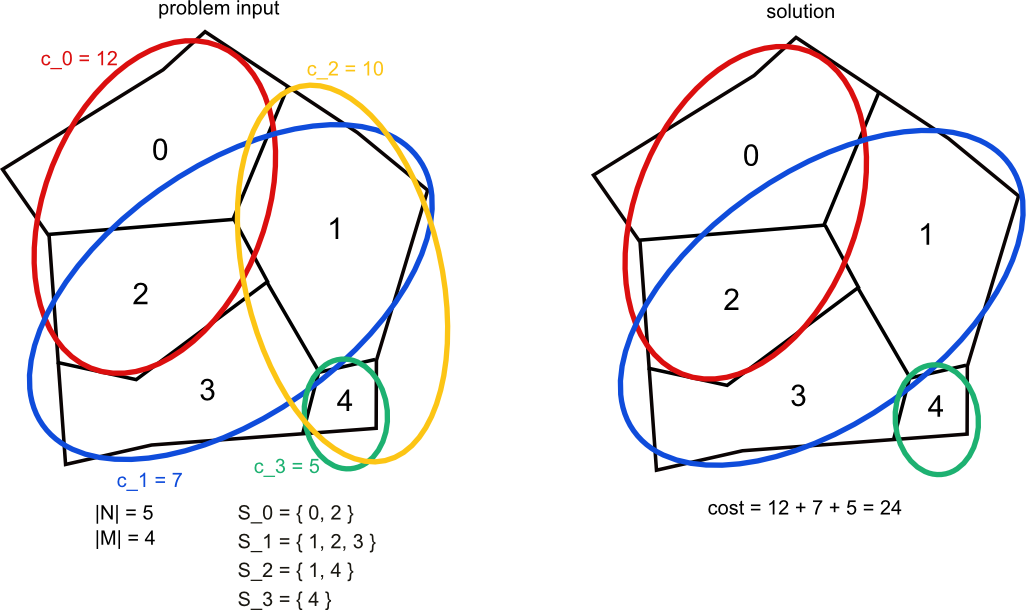
\includegraphics[width=14.0cm]{figures/setCover.png}
%        \begin{subfigure}[b]{8.0cm}%{0.3\textwidth}
%                \centering
%                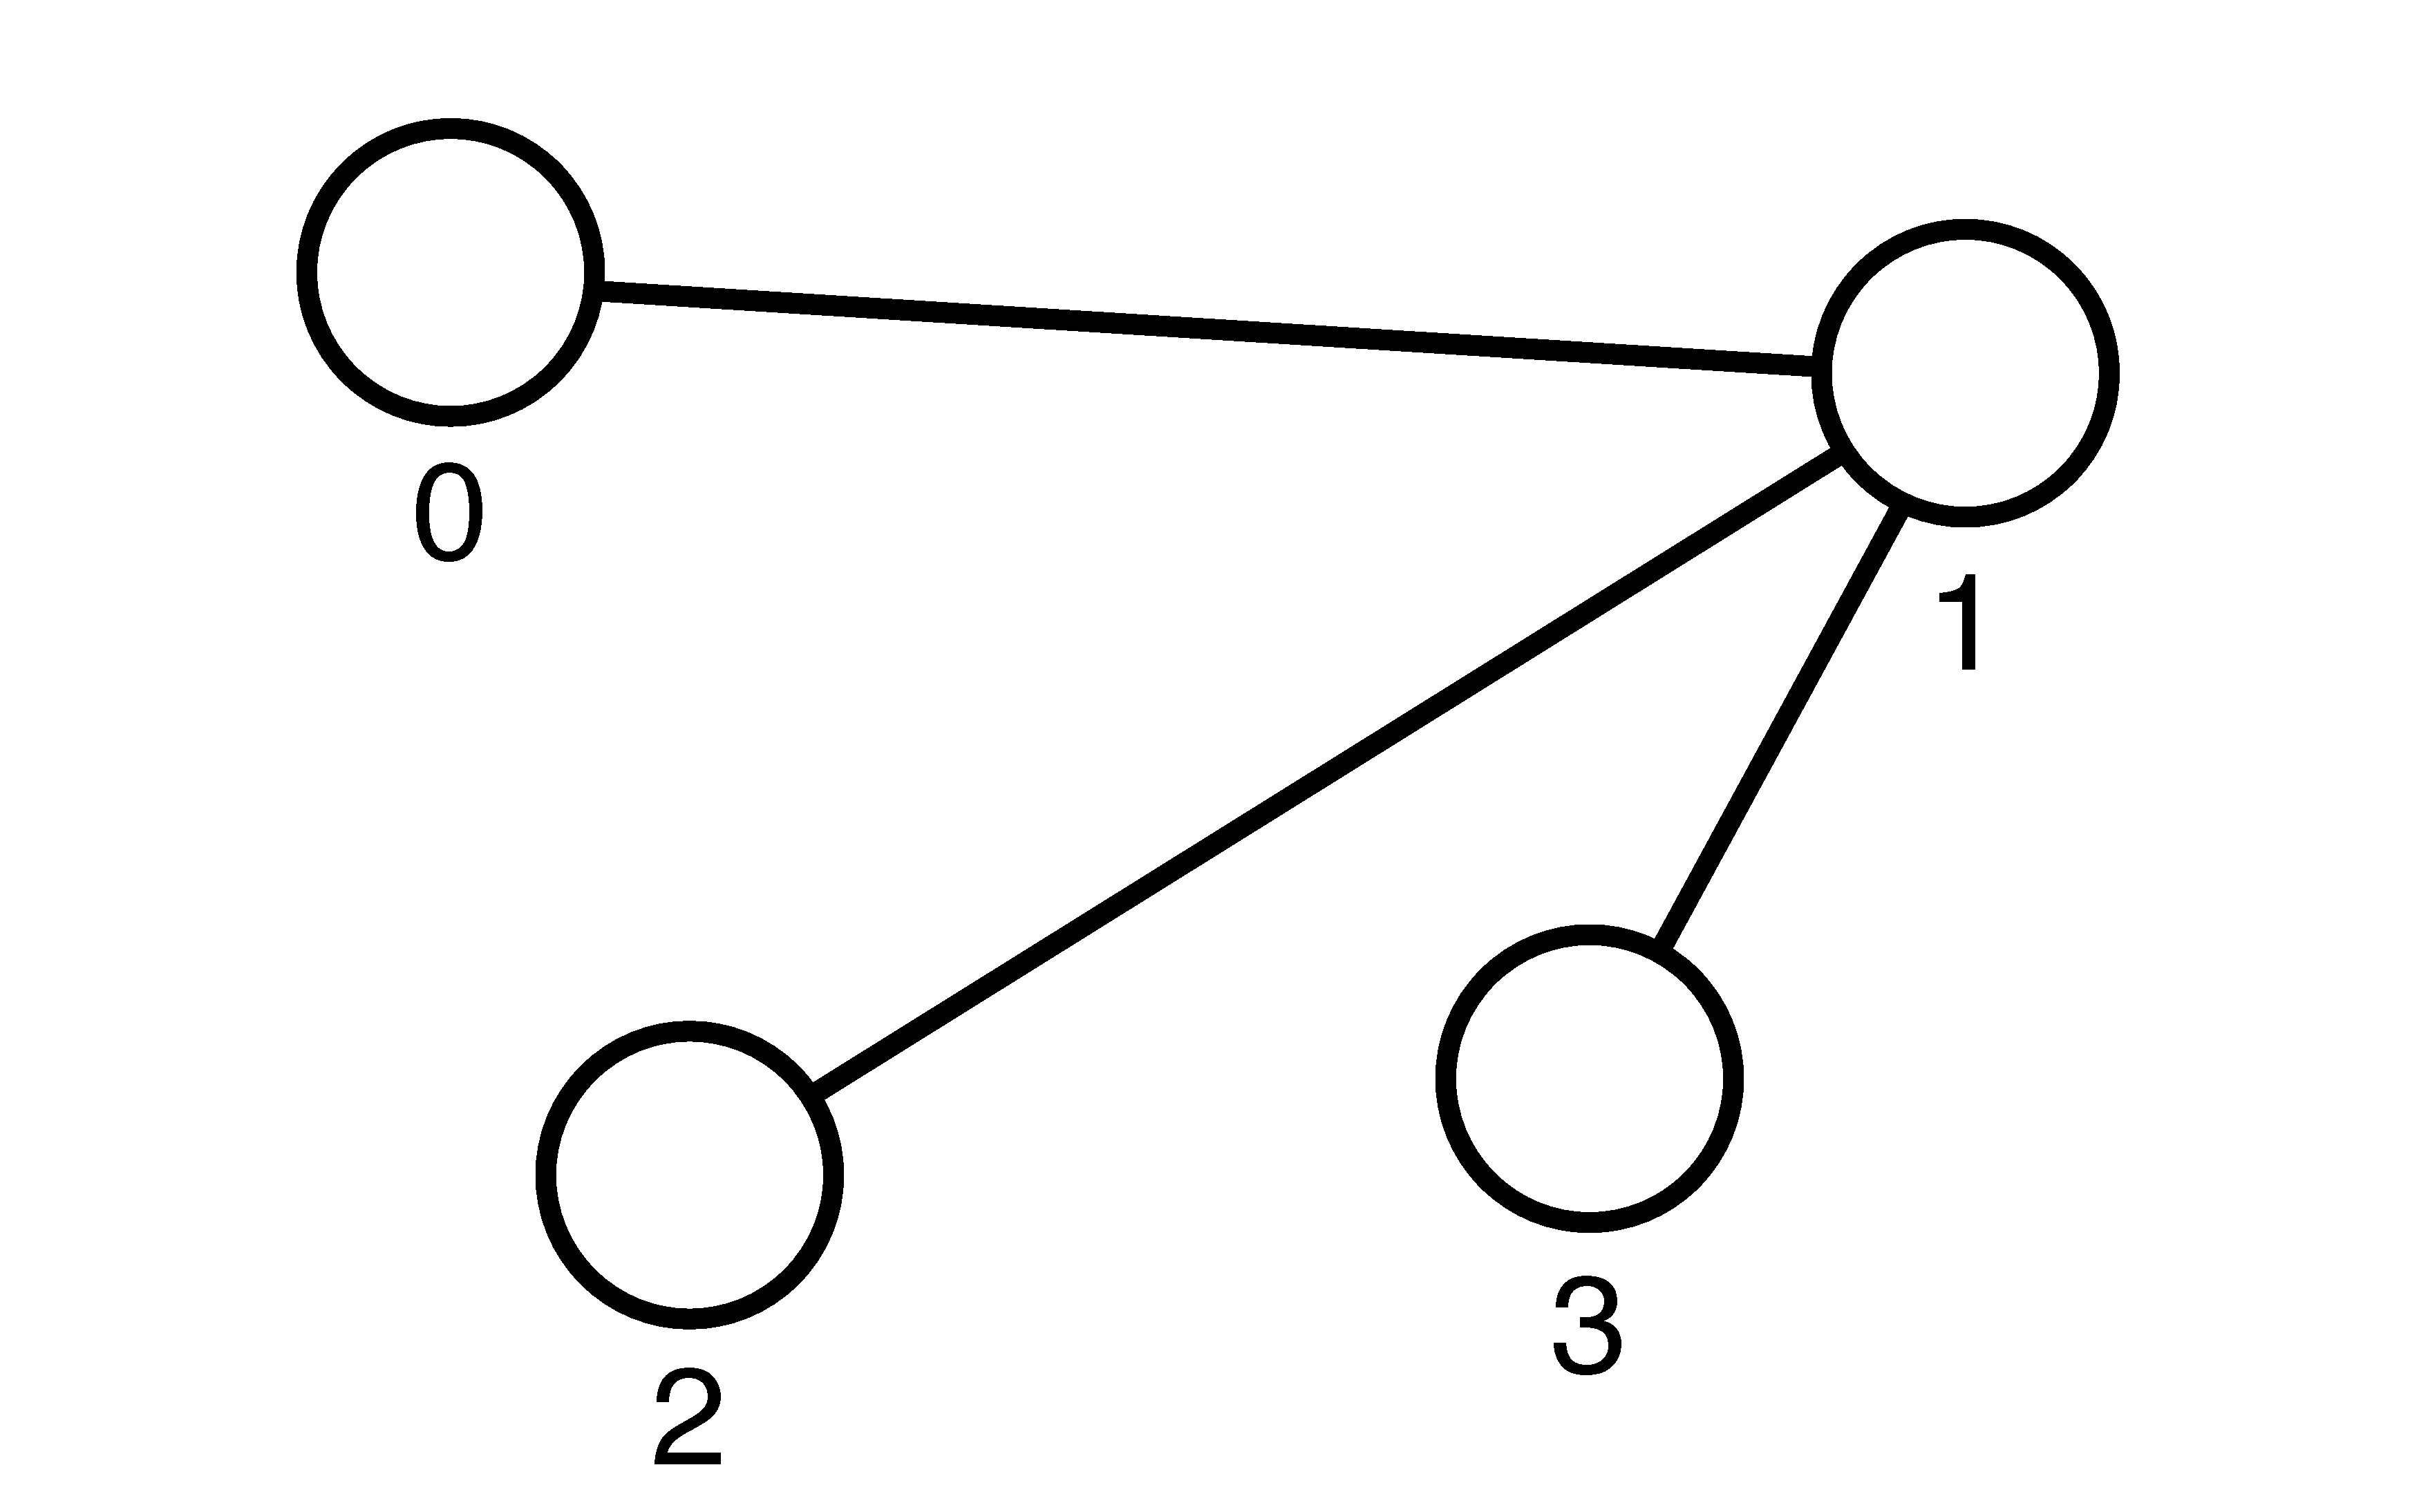
\includegraphics[width=8cm]{figures/coloring_1.pdf}
%                \caption{A graph.}
%                \label{fig:graph:input}
%        \end{subfigure}%
%        ~ %add desired spacing between images, e. g. ~, \quad, \qquad etc.
%          %(or a blank line to force the subfigure onto a new line)
%        \begin{subfigure}[b]{8.0cm}
%                \centering
%                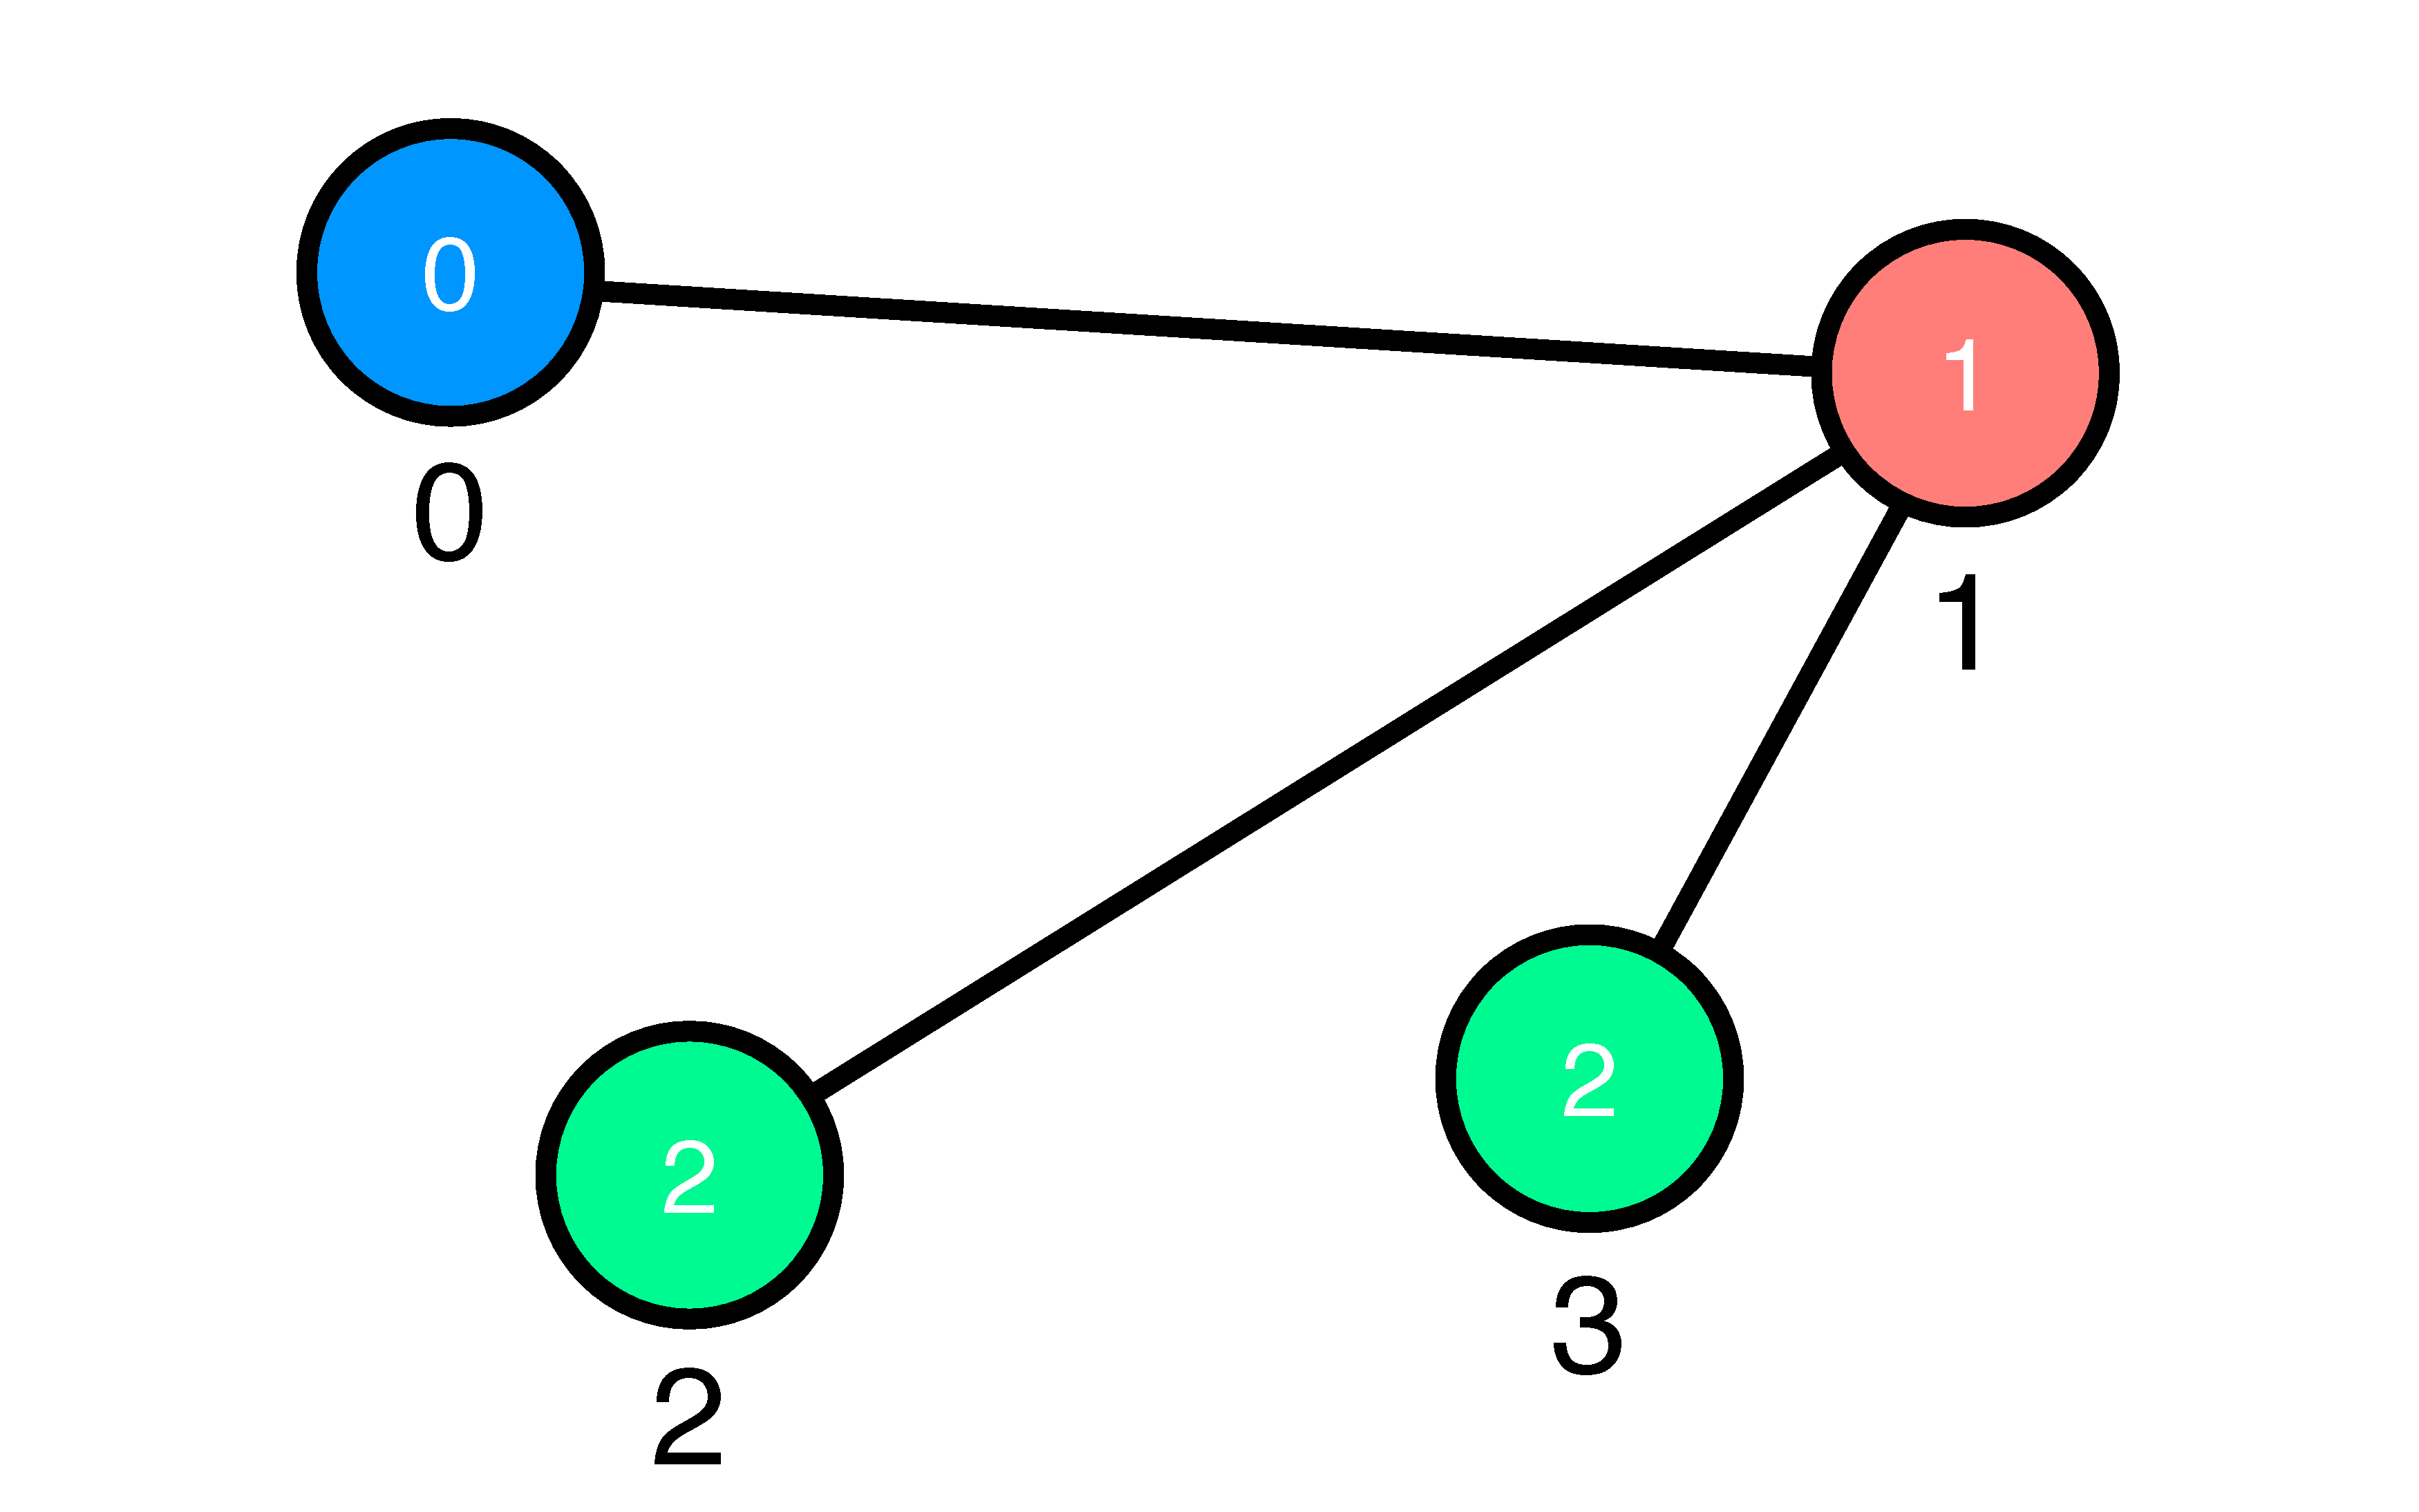
\includegraphics[width=8cm]{figures/coloring_2.pdf}
%                \caption{A three-coloring of the graph.}
%                \label{fig:graph:coloring}
%        \end{subfigure}
\caption{A Set Cover Example}\label{fig:graph}
\end{figure}

\section{Assignment}

Write an algorithm to solve the set cover problem. We will now generalise the problem 
and therefore call the regions `{\em items}' and the fire-stations `{\em sets}'. 
The problem is mathematically formulated 
in the following way: We are given a number of items (regions) $N = \{0 \dots n-1\}$ and  
sets (possible fire-stations) $M = \{0 \dots m-1\}$. 
For each set $i \in M$, we know the cost $c_i$, and the set of items $S_i \subseteq N$ that 
it covers. For instance,
in Fig.~\ref{fig:graph}, the first possible fire-station has cost $c_0 = 12$ and covers 
regions $S_0 = \{0,2\}$.
We use variables $x_i \in \{0,1\}$ to denote if we select set $i$. Our goal is to find a
selection of sets with minimal cost that cover all items. 
The set cover problem is formalized as the following optimization problem,

%Introduce the input data, useful sets, and decision variables.  Formalize the problem as a declarative optimization model.

$$
\begin{array}{ll}
\mbox{minimize:} & \displaystyle \sum_{i \in M} c_i x_i \\
\mbox{subject to:} & \\
     & \displaystyle \sum_{i \in M} (j \in S_i)x_i \geq 1 \;\;\; (j \in N)\\
     & x_i \in \{0,1\}\\
\end{array}
$$
%
where the constraint ensures that each item is covered at least once: for each item $j \in N$, 
it states that the sum over all sets $i \in M$ that contain item $j$, has to be greater or 
equal to 1. 

%\clearpage
\section{Data Format Specification}

The input consists of $|M|+1$ lines, where $|M|$ is the number of sets. 
The first line contains 2 numbers: the number of items, $|N|$, and the number of 
sets, $|M|$. It is followed by $|M|$ lines, where each line represents 
the data for a set $i$: first comes the cost $c_i$, followed by the
items  $S_i = \{ s_{i0}, s_{i1}, \dots \}$ that set $i$ covers.

\vspace{0.2cm}
\noindent
Input Format
\vspace{-0.2cm}
\begin{Verbatim}[frame=single]
|N| |M|
c_0 s_0_0 s_0_1 ...
c_1 s_1_0 s_1_1 ...
c_2 s_2_0 s_2_1 ...
...
c_|M|-1 s_(|M|-1)_0  ...
\end{Verbatim}
%
%
The output has two lines.  The first line contains two values $obj$ and $opt$.  $obj$ is the cost of the selected sets (i.e. the objective value).  $opt$ should be $1$ if your algorithm proved optimality and $0$ otherwise.  The next line is a list of $|M|$ values in $\{0,1\}$, one for each of the $x_i$ variables that represent which sets have been selected.  This line encodes the solution.
\vspace{0.2cm}
\noindent
Output Format
\vspace{-0.2cm}
\begin{Verbatim}[frame=single]
obj opt
x_0 x_1 ... x_|M|-1
\end{Verbatim}
%
%It is essential that the value order in the solution output matches the value order of the input.  Otherwise the grader will misinterpret the output.

\clearpage
\paragraph{Examples}
%\vspace{0.1cm}
%\noindent
%(based on Figure \ref{fig:graph})
(based on Figure \ref{fig:graph})

\vspace{0.2cm}
\noindent
Input Example
\vspace{-0.2cm}
\begin{Verbatim}[frame=single]
5 4
12.0 0 2
7.0 1 2 3
10.0 1 4 
5.0 4
\end{Verbatim}

\vspace{0.2cm}
\noindent
Output Example
\vspace{-0.2cm}
\begin{Verbatim}[frame=single]
24.0 0
1 1 0 1
\end{Verbatim}
%
The output example illustrates the problem input and solution from Figure \ref{fig:graph}.

\section{Instructions}

Edit \texttt{solver.py} and modify the \texttt{solve\_it(input\_data)} function to solve the optimization problem described above.  The function argument, \texttt{input\_data}, contains the problem data in the format described above.  The return value of \texttt{solve\_it} is a solution to the problem in the output format described above.  Your \texttt{solve\_it} implementation can be tested with the command, 
\[ 
\texttt{python ./solver.py ./data/<inputFileName>} 
\] 
You should limit the \texttt{solve\_it} method to terminate within 5 hours, otherwise the submission will not be eligible for full credit.  You may choose to implement your solver directly in python or modify the \texttt{solve\_it} function to call an external application.

%We use \texttt{stdout} for output.
%Output to other stream will be ignored (you may want to send runtime information to \texttt{stderr}). Your submission will be tested on a department linux machine. If your algorithm is a standalone program, please name it \texttt{nr},
%otherwise, please specify the compilation procedure,
%it is appreciated if you also provide a script that follows the above format to run the program.

\paragraph{Resources}
You will find several set covering problem instances in the \texttt{data} directory provided with the handout.

%An example output file, \texttt{blabla.out}, is also provided.

%\section{Remarks}

\paragraph{Handin}
Run \texttt{submit.py} with the command, \texttt{python ./submit.py}.  Follow the instructions to apply your  \texttt{solve\_it} method on the various assignment parts.  You can submit multiple times and your grade will be the best of all submissions.  However, it may take several minutes before your assignment is graded; please be patient.  You can track the status of your submission on the {\em feedback} section of the assignment website.


\paragraph{Grading}
Infeasible solutions (i.e. those that do not conform to the output format or violate problem constraints) will receive 0 points.  Feasible solutions will receive at least 3 points.  Feasible solutions passing a low quality bar will receive at least 7 points and solutions meeting a high quality bar will receive all 10 points.  The grading feedback indicates how much your solution must improve to receive a higher grade.


%\paragraph{Collaboration Rules} 

In all assignments we encourage collaboration and the exchange of ideas on the discussion forums.  However, please refrain from the following:
\begin{enumerate}
\item Posting code or pseudo-code related to the assignments.
\item Using code which is not your own.
\item Posting or sharing problem solutions.
\end{enumerate}
Discussion of solution quality (i.e. objective value) and algorithm performance (i.e. run time) is allowed and the assignment leader board is designed to encourage such discussions.

\paragraph{Collaboration Rules} 

In open source assignments we encourage collaboration, exchange of ideas, and code!  However, please refrain from the following:
\begin{enumerate}
\item Posting or sharing problem solutions.
\end{enumerate}
The goal here is to share your algorithms, not just a list of high quality solutions.


%\paragraph{Questions} Please contact the class GTA Carleton (cjc@cs.brown.edu).

\paragraph{Warnings} 

\begin{enumerate}
\item It is recommended you do not modify the \texttt{data} directory.  Modifying the files in the data directory risks
making your assignment submissions incorrect.
\item You cannot rename the \texttt{solver.py} file or the \texttt{solve\_it()} method.
\item Be careful when using global variables in your implementation.  The \texttt{solve\_it()} method will be run repeatedly and it is your job to clear the global data between runs.
\item \texttt{solver.py} must remain in the same directory as \texttt{submit.py}.
\end{enumerate}


%\paragraph{Hint} 
%The optimal value for  \texttt{data/gc\_1000\_5} is near $85$.
 
\section{Technical Requirements}

You will need to have python 2.7.x or 3.5.x installed on your system (installation instructions, \\ \texttt{\url{http://www.python.org/downloads/}}).


\end{document}




